\documentclass[12pt, a4paper]{article}
\usepackage{enumitem, amssymb }
\usepackage{fancyhdr}
\usepackage{graphicx}
\usepackage[english]{babel}
\usepackage{listings}
\usepackage{color}
\usepackage{fontspec} 
\usepackage{hyperref}

\lstset{basicstyle=\footnotesize\ttfamily,breaklines=true}
\lstset{framextopmargin=50pt,frame=bottomline}
\date{2020-6-16}
\author{Ebbe Vang}
\title{IDS Kit}
\pagestyle{fancy}
\fancyhf{}
\setlength{\headheight}{15pt}
\rhead{
\includegraphics[height=10pt]{RUC_BLACK_RGB.png}}
\lhead{Interactive Digital Systems}
\cfoot{\thepage}
\newlist{todolist}{itemize}{2}
\setlist[todolist]{label=$\square$}
\setmainfont{Arial}
\definecolor{mygreen}{rgb}{0,0.6,0}
\definecolor{mygray}{rgb}{0.5,0.5,0.5}
\definecolor{mymauve}{rgb}{0.58,0,0.82}


\lstset{ %
language=c++,
numbers=left,
backgroundcolor=\color{white},   % choose the background color
basicstyle=\footnotesize,        % size of fonts used for the code
breaklines=true,                 % automatic line breaking only at whitespace
captionpos=b,                    % sets the caption-position to bottom
commentstyle=\color{mygreen},    % comment style
escapeinside={\%*}{*)},          % if you want to add LaTeX within your code
keywordstyle=\color{blue},       % keyword style
stringstyle=\color{mymauve},     % string literal style
}

\begin{document}



\section{Content of the electronics kit}  

You borrow your kit personally from FlexLab and it must be handed back to
FlexLab at the end of the course.

When handing out, please check the contents with this list and
let us know if anything is missing. When handing in the kit, we also ask
you to check the contents and make us aware if you
have lost something or something is defective.
\begin{todolist}
  \item ESP32 Development Board
  \item 2 Breadboards (830 Point Solderless and Transparent)
  \item 2 Joysticks
  \item Potentiometer with cap
  \item GY-521 Accelerometer 
  \item Character LCD /w IIC/I2C Serial Interface Adapter
  \item 0.91inch OLED LCD Display Module 128x32 I2C 
  \item Micro USB Cable
  \item 3 push buttons
  \item Piezo Electronic Buzzer Alarm 95DB
  \item Small Toggle Switch Interruptor
  \item Cable Bundle
  \item various colored LEDs
  \item resistor
  \item RGB LED
\end{todolist}

%\section{about the Esp32 microcontroller}  

%\subsection{GPIO pins}

%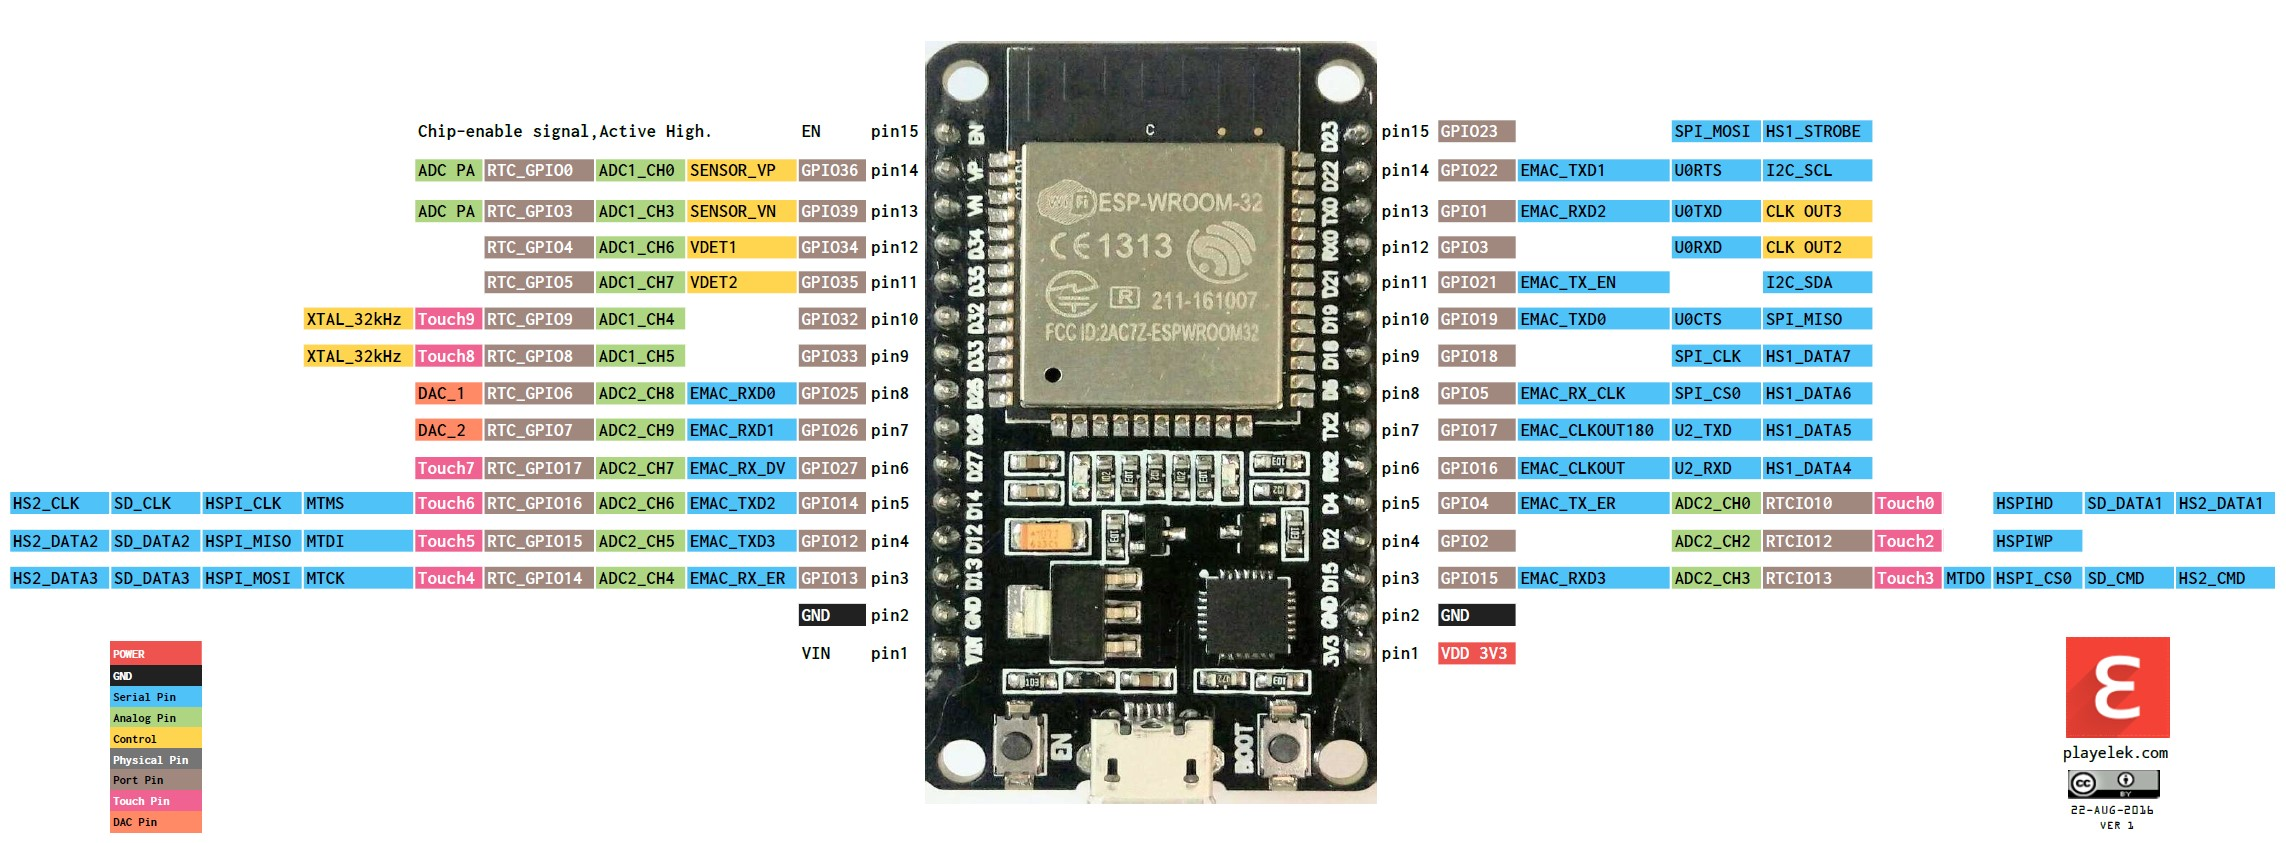
\includegraphics[width=\textwidth,keepaspectratio=true]{ESP32Espresiffboards12.jpg}

\newpage
\section{Reading the pins on our microscontroller}

\subsection{Digital Input / Output}

In these first examples, we try to keep things simple and concentrate on controlling a single pin (LED) in the first example and then reading a pin (button) 
in the next example. In these examples we use digital input / output. 
Either there is power on the stick or there is not. 
Later in the next section we try with analog inputs and outputs, such as reading the resistance in a potentiometer or being able to control the brightness of an LED.

\subsubsection{Blink example}
The Blink example can be described as the "hello world"-script for microprocessors. Pay attention to the first line where we include arduino, this line of code is only necessary because we use platoformIO as our editor. If you search the net for blink or other arduino examples you will often find examples where this line is missing. That is because the arduino IDE add that by itself.

The code will only work if you connect a LED to pin number 15 and GND.

\lstinputlisting{code_examples/lecture_1/led.cpp}

\subsubsection{Button Example using 'Pullup'}

This example introduces digtialRead() and demonstrate the use og a built in pullup resistor. 
The reason we use it the pullup resistor is to avoid that the voltage is fluctiating when the button isn't connected to the ground(gnd)

\lstinputlisting{code_examples/lecture_1/button.cpp}

\subsection{Analog Input}
in previous examples we work with the digitalread function to check if there was power on a pin or not. But many sensors work differently. They are not just on or off but provide a value that can vary between 0 and 4095 (by default on an ESP32)

We will now look at an example where we read a potentiometer. you can change the setting on the potentiometer and read a changing value in our serial monitor

When you run the sample you should be able to see a changing value being printed in your serial monitor. When you turn the potentiometer, the value should change. Even when you are not touching the potentiometer we must expect the value to change a bit because the voltage always fluctuates a little bit.

It's time to set up your electrical circuit and test the example:
\begin{center}
  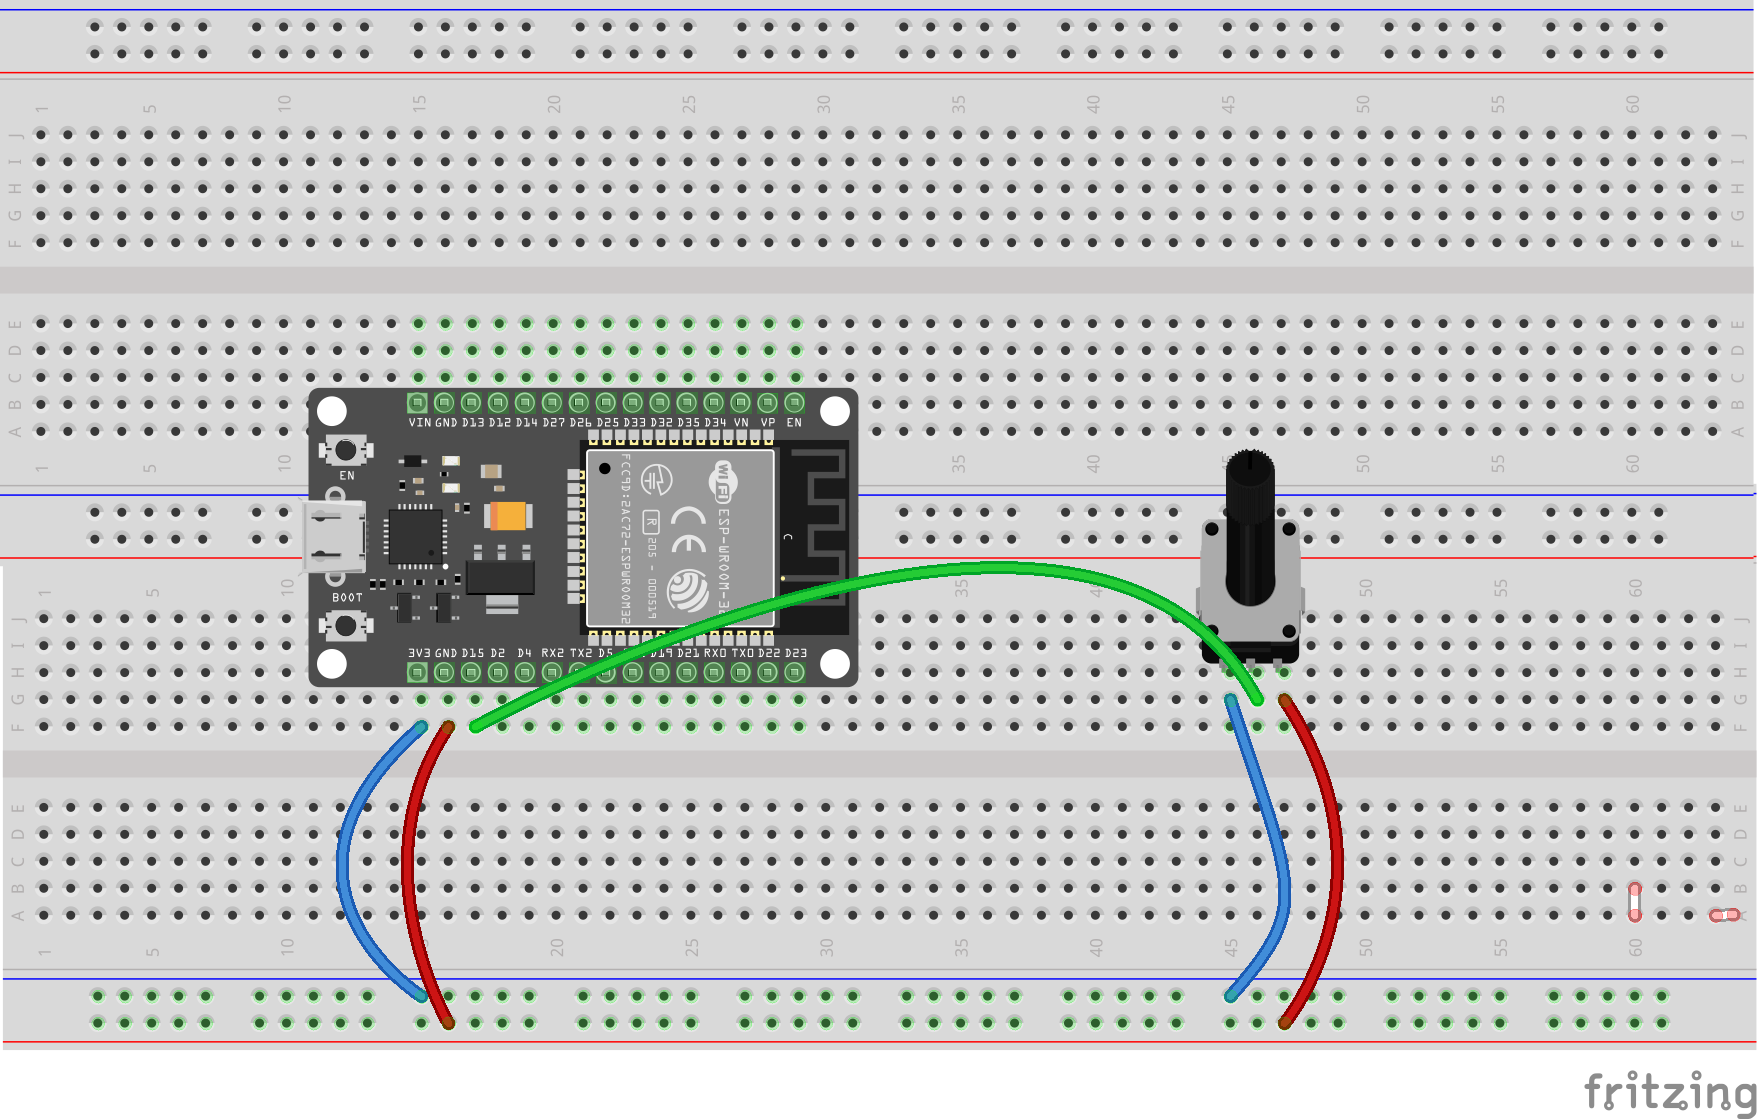
\includegraphics[width=12cm, keepaspectratio]{fritzing/analogInput_potentiometer.png}
\end{center}

\lstinputlisting{code_examples/lecture_2/analogread_potentiometer.cpp}

programs above show a number between 0 and 4095. the number tells how big the voltage is on the pin we are measuring. Let's change the code a bit so it shows how many volts there are on our pin. we insert a small calculation where we calculate volts based on the ESP32 emitting 3.3v and our range is from 0-4095:

\lstinputlisting{code_examples/lecture_2/analogRead_voltage.cpp}

\subsubsection{PWM: Power with modulation}

Now we have looked at how to read analog input using the analogRead () function. When we want to control output, a technique called PWM is used. The principle is that we turn the power on and off very quickly. Then the "voltage" is controlled by how long the power is on in relation to how long it is off.
You set a duty cycle that determines how much of the time we turn on the power, and frequency which sets the speed for how often we want to "turn on and off" the power.

See example below:
\begin{center}
  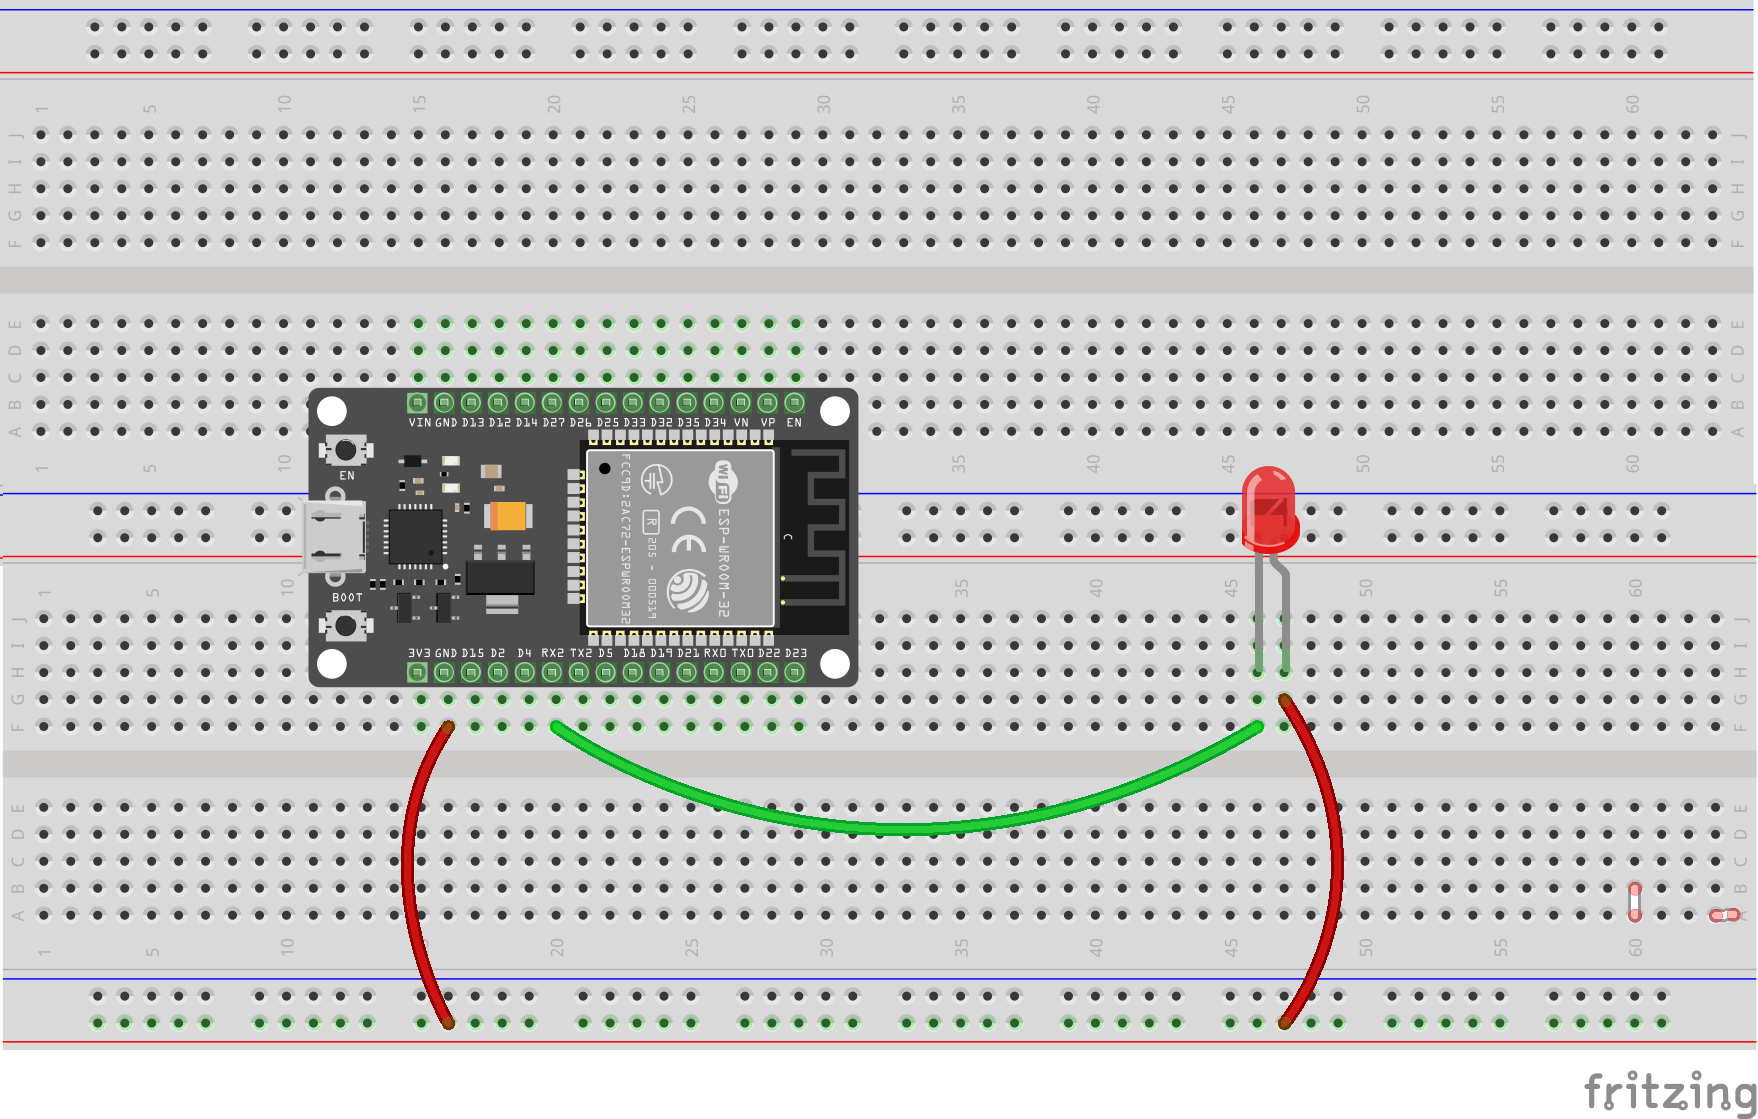
\includegraphics[width=12cm, keepaspectratio]{fritzing/pwm_led.png}
\end{center}


\lstinputlisting{code_examples/lecture_2/pwm_led.cpp}

\end{document}